\documentclass[runningheads,a4paper]{llncs}
\usepackage{amssymb}
\usepackage{url}
\usepackage{hyperref}
\usepackage{times}
\usepackage{float}
\usepackage{inconsolata}
\usepackage[T1]{fontenc}
\usepackage{graphicx}
\usepackage{color}
\usepackage{soul}  
\usepackage{nameref}  
\usepackage{amsbsy}  
\usepackage{bezier}  
\usepackage{colortbl}  
\usepackage[leqno,fleqn]{amsmath}  
\usepackage{verbatim}
\usepackage{multicol}
\usepackage{wrapfig}
% deutsche Silbentrennung
\usepackage[ngerman]{babel}
% wegen deutschen Umlauten
\usepackage[utf8]{inputenc}
\usepackage{listings}
\usepackage{epstopdf}

\lstloadlanguages{Ruby}
\lstset{%
  basicstyle=\fontfamily{fi4}\selectfont\color{black},
  commentstyle = \fontfamily{fi4}\selectfont\color{red},
  keywordstyle=\fontfamily{fi4}\selectfont\color{blue},
  stringstyle=\color{green},
  language=Ruby,
  basicstyle=\footnotesize,      % font size
  numbers=left,                  % where to put line numbers
  numberstyle=\footnotesize,     % numbers size
  numbersep=5pt,                 % how far the line numbers are from the code
  backgroundcolor=\color{white}, % background color
  showspaces=false,                          % show spaces (with underscores)
  showstringspaces=false,            % underline spaces within strings
  showtabs=false,                            % show tabs using underscores
  frame=tb,                  % adds a frame around the code
  tabsize=2,                     % default tabsize
  breaklines=true,                  % automatic line breaking
  columns=fullflexible,
  breakautoindent=false,
  framerule=1pt,
  xleftmargin=0pt,
  xrightmargin=0pt,
  breakindent=0pt,
  resetmargins=true,
  stepnumber=1
}


\setcounter{tocdepth}{3}
\newcommand{\keywords}[1]{\par\addvspace\baselineskip
\noindent\keywordname\enspace\ignorespaces#1}

\begin{document}
\mainmatter

\title{Behaviour Driven Development}
\subtitle{Proseminar - Systemanalyse und -design}
\date{Sommersemester 2013}

\author{Steve Dierker}

\institute{
Freie Universit\"at Berlin\\ Institut for Computer Science \\ AG Corporate Semantic Web \\
K\"onigin-Luise-Str. 24/26, 14195 Berlin, Germany\\  dierker.steve@fu-berlin.de \\
\url{http://www.inf.fu-berlin.de/ag-csw}
}

\maketitle

\begin{abstract}
  In dieser Seminararbeit geht es um Behaviour Driven Developent als Sofware 
  Prozess. Insbesondere werden wir uns mit den Gr"unden f"ur die Entwicklung von
  Behaviour Driven Development und den Vor- und Nachteilen zu klassischem Test 
  Driven Development besch"aftigen.\\
  Ein besonderer Fokus wird hier auf ausgew"ahlten Werkzeugen zur Umsetzung von 
  BDD mit der Programmiersprache {\em Ruby} gelegt.
\end{abstract}

\keywords{Behaviour Driven Development, Agile Software Process, Ruby, Seminararbeit}

\section{Einleitung}
  BDD ist eine Weiterentwicklung von Test Driven Development und Verkn"upfung 
  mit anderen bestehenden agilen Software Processen wie Domain Driven Design 
  und Object Oriented Analysis.\\
  Programmierer die das erste mal mit TDD in Ber"uhrung kommen brauchen eine 
  lange aufw"arm Phase bis sie effektiv mit diesem Konzept arbeiten k"onnen. 
  Denn bei der Verfolgung dieses Konzeptes stellen sich als erstes zwar simpel 
  erscheinende doch sehr wichtige Fragen.\\
  \begin{itemize}
    \item Was soll getestet werden?
    \item Wo f"angt man mit dem Testen an?
    \item Wieviel sollte ein Test "uberhaupt testen?
    \item Wie sollten Tests benannt sein?
    \item Wie sollte verstanden werden warum ein Test fehlschl"agt?
  \end{itemize}
  Diese Fragen f"uhren zu einer starken Diversit"at zwischen den Umsetzungen
  der Idee von TDD zwischen vielen Programmierer\_innen und erschwert es das Konzept
  schnell und klar an andere Entwickler\_innen weiter zu vermitteln.\\
  Es braucht also eine klar Struktur von 'Best Practises' f"ur TDD um den 
  Umgang mit diesem Prozess zu vereinheitlichen und Anf"angern die M"oglichkeit
  zu geben auch ohne Vorkenntnisse schnell in bestehende Projekt mit diesem 
  Prozess einzusteigen.\\
  Genau diese Probleme, die von Programmierer\_innen die Erfahrung im Umgang mit TDD 
  haben meist umgangen werden indem sie "ahnliche konzeptionelle Methoden wie 
  BDD verfolgen, wurden von Dan North\cite{North:2006} in seinem 
  Artikel erstmals zusammengefasst.\\
  Genau auf diese Konzepte werde ich n"aher eingehen.
\section{Test Driven Development}
  Bevor wir in BDD eintauchen k"onnen m"ussen wir verstehen wie Test Driven 
  Development funktioniert, welche Vorteile es uns bringt und auf welche 
  Probleme wir sto"sen k"onnen.

  \subsection{Red-Green-Refactor}
    Grundlegend ist TDD ein Software Desing Process. Dieser Prozess basiert auf 
    der klaren Mantrik erst Tests f"ur einen nicht existenten Codeabschnitt zu
    schreiben, bevor der Code selbst implementiert wird.\\
    \begin{wrapfigure}{r}{0.5\textwidth}
      \vspace{-30pt}
      \begin{center}
        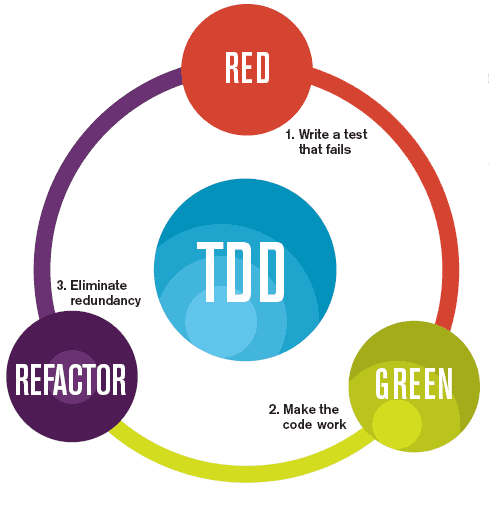
\includegraphics[scale=0.3]{assets/tdd_flow.png}
      \end{center}
      \caption{Red-Green-Refactor\cite{Osorio:2012}}
      \vspace{-15pt}
    \end{wrapfigure}
    Dies wird auch oft als 'Red-Green-Refactor-Zyklus' bezeichnet, da erst der Test
    ausgef"uhrt wird und fehlschl"agt, was bei den meisten Testingframeworks mit 
    Rot markiert wird, nun das Feature implementiert wird und der Test nicht 
    fehlschl"agt -dies wird oft mit Gr"un dargestellt.\\
    Sobald der Test nicht mehr feschl"agt betrachtet man das entstandene Design 
    des Features, reduziert Duplikate und kommentiert seinen Code. Nun kann man 
    ein weiteres mal in den Zyklus eintreten und die n"achsten Features wieder 
    nach dem gleichen System entwickeln.\\
    Ein Zyklus sollte allerdings nicht l"anger als 15 Minuten dauern. Falls doch
    hei"st dies entweder das zu implementierende Feature ist zu gro"s gew"ahlt
    oder der gew"ahlte L"osungsweg nicht optimal ist. Generell 
    sollten sich die Entwickler\_innen immer die Frage stellen ob Debuggen 
    schneller als neu implementieren eines Features ist, solange die Tests bei erst
    Implementierung fehlschlagen.

  \subsection{Auswirkungen und Vorteile}
    Sobald die Codebase w"achst wird immer mehr Zeit zum umstrukturieren des 
    bereits entwickelten Quellcodes ben"otigt und es wird sich langsam ein 
    sich konstant weiterentwickelndes Design herauskristallisieren.\\
    Durch diese evolvierende Art des Designs, auch 'Emergent Design'\cite[p.~4]{Chelimsky:2010} genannt, kann sich die Software und somit auch die 
    Entwickler\_innen dynamisch den Anforderungen des Stakeholders anpassen, was 
    besonders in agilen Softwareprozessen n"otig ist. Des weiteren ist es auf 
    Grund der 'Test First' Struktur stets m"oglich ein zumindest begrenzt 
    fertiges Produkt zu pr"asentieren, was sofortige Kommunikation und Feedback
    des Stakeholders erm"oglicht und schnell aufkommende Probleme in der Software
    sichtbar werden l"asst.\\

  \subsection{Bestehende und absehbare Probleme}
    Test Driven Development sollte nicht als Ersatz eines ausf"uhrlichen Testens
    der Software gesehen werden. Eher ist es als Prozess zusehen um qualitativen
    Quellcode an den der Entwicklung angeschlossenen Testzyklus zu "ubergeben.\\
    Doch genau das f"uhrt schnell zur Verwirrungen, da Entwickler\_innen dazu
    neigen TDD als M"oglichkeit zusehen sich diesen extra Testzyklus zu sparen.
    Dies f"uhrt dazu das w"ahrend des Entwickelns neuer Features nicht nur 
    Tests geschrieben werden die das Verhalten des Features nach au"sen spezifizieren
    sondern interne technische Details auf Funktion "uberpfr"ufen. Dadurch werden
    die Tests besonders von unerfahrenen TDD-Entwickler\_innen schnell zu 
    ausf"uhrlichem White-Box-Testing genutzt, was zu einer starken Verschr"ankung
    von Test-Suite und eigentlich Quellcode f"uhrt. Durch diese Verschr"ankung
    wird das im Zyklus enthaltene Umstrukturieren des Codes immer weiter 
    erschwert und die Test-Suite verliert an Wartbarkeit, da f"ur das von au"sen
    betrachtete Verhalten unwichtige technische Details bei "Anderungen zum 
    fehlschlagen der Tests f"uhren k"onnen.\\
    Speziell hierf"ur m"ussen die Entwickler\_innen Disziplin an den Tag legen,
    denn sie sind es die das "aussere Verhalten als Test implementieren und sich
    selbst davon abhalten m"ussen internes Verhalten zu testen.\\
    Ein strukturelles Problem bei TDD ist es, das die Entwickler\_innen selbst
    die Anforderungen der Stakeholder in Tests "ubersetzen m"ussen und es 
    dadurch dazu kommen kann das schon die Tests falsches verhalten pr"ufen
    und somit die Implementierung des Features gar nicht den Anforderungen 
    entsprechen kann. Au"serdem folgt aus der nicht klar gegebenen Nomenklatur
    f"ur Tests, dass sie zwar auf Grund ihrer Funktion das Verhalten der 
    Software dokumentieren, dies allerdings nur auf einer f"ur Entwickler\_innen
    lesbaren Ebene, obwohl nur der Stakeholder verifizieren k"onnnte, das die 
    Tests sein gew"unschtes Verhalten abdecken. Dies kann vielleicht durch 
    Erfahrung der Entwickler\_innen ausgeglichen werden indem sie klare 
    Methodennamen vergeben und durch viele Kommentare auch Menschen die nicht 
    im Programmieren bewandert sind die M"oglichkeit geben die Tests zu 
    verstehen.\\
    Allerdings muss nun jedes neue Teammitglied an diese speziellen Verfahren
    gew"ohnt werden, da sie auf Grund mangelnder Einheitlichkeit stark zwischen
    verschiedenen Teams varieren k"onnen.
    Ausserdem stellt sich f"ur die Entwickler immer die Frage bei welchem Feature
    sie nun mit Tests und Implementierung starten sollte, da sie ja nur die 
    "Ubersicht "uber alle Anforderungen des Stakeholders haben. Hierbei kann man
    als Richtlinie angeben das man von klein nach gro"s entwickeln sollte und 
    immer auf Funktionst"uchtigkeit des entstehenden Quellcodes achten sollte.\\
    Bei der Entwicklung eines Onlineshops f"angt man zum Beispiel als erstes 
    an Artikel einpflegen zu k"onnen, ohne Beachtung dessen das das nur f"ur
    Administratoren m"oglich sein sollte und erst sp"ater in der Entwicklung
    f"ugt man das Feature f"ur Logins hinzu.\\
    Es wird also eine inkrementelle Entwicklung gef"ordert, allerdings ben"otigt
    diese Erfahrung um sich nicht in Sackgassen in der Entwicklung zu verrennen.\\
\section{Behaviour Driven Development}
  Beavhiour Driven Development basiert auf den Ideen von TDD und erweitert diese
  um wichtige Namenskonventionen und Begriffe, sodass klarer wird welche Schritte
  wie als Programmierer\_inn zu befolgen sind um qualitativ hochwertige Software
  zu entwickeln.\\
  Diese Erweiterung f"uhrt neue Begriffe und Werkzeuge in vier Bereichen
  \begin{itemize}
    \item Vokabular
    \item Frameworks
    \item Methodik
    \item User-Stories
  \end{itemize}
  in den TDD Zyklus ein und f"ugt einen TDD umfassenden Zyklus hinzu.

  \subsection{Unterschiede zu Test Driven Development}
    \subsubsection{Vokabular}
      ist der gr"o"ste Unterschied zu TDD. Denn bei BDD
      ist der Fokus wie der Name schon sagt auf 'Behaviour (Verhalten)' der 
      Software gelegt. Dadurch wird den Entwickler\_innen klarer deutlich
      das es in diesem Entwicklungsprozess nicht um vorzeitiges ausf"uhrliches
      White-Box-Testing einer Software geht, sondern um ein vom gew"unschten 
      Verhalten der Software getriebenes Design.\\
      In BDD wird daher nicht als erstes die Struktur des Quellcodes durch die 
      Entwickler\_innen durch Tests gepr"uft, sondern auf das gew"unschte
      Verhalten der Software von au"sen eingegangen. Hierzu werden zusammen
      mit den Stakeholdern User-Stories in Form der {\em Gherkin}\cite{Gherkin} Sprache verfasst, die
      dann automatisiert in Verhaltenstest der Software umgewandelt werden.
      Dadurch ist es m"oglich das die Stakeholder schnell und einfach das 
      Verhalten gew"unschte Verhalten ihrer Software definieren k"onnen und
      die Entwickler\_innen nun gegen dieses Verhalten entwickeln.\\
      Die {\em Gherkin-Sprache} ist in einer Englisch nahen Syntax 
      gehalten und basiert im Grunde auf den drei Stichw"ortern 'Given', 'When' 
      und 'Then'. Nun wird in simplen englischen S"atzen definiert welche 
      Vorbedingung gelten sollten ('given'), durch welche Ereignisse die 
      Nachbedingung erforderlich wird ('when') und welche Nachbedingung gelten
      sollte ('then'). Dadurch ist es nun den Stakeholdern m"oglich direkt 
      das gew"unschte Verhalten zu spezifizieren.\\
      Hier ist dies ein BDD-Feature f"ur einen einfachen Taschenrechner, welches
      nur das Verhalten f"ur Multiplikationen definiert. Wie zusehen ist, ist 
      es ohne extensive Vorkenntnisse m"oglich Features in {\em Gherkin} zu spezifizieren.
      \lstinputlisting[caption=Gherkin Beispiel ({\em Ruby} Cucumber)]{../features/multiplication.feature}
      Nat"urlich stellt sich nun die Frage wie aus diesem leicht strukturierten
      Flie"stext automatisiert Testf"alle f"ur die Entwickler\_innen erstellt werden.
      Dies l"ost {\em Cucumber}\cite{Cucumber}, ein BDD Framework f"ur {\em Ruby}, in dem die Entwickler\_innen durch Definition kleiner Regex-Schritte angeben 
      welches Satz Schema welche Bedeutung hat.
      \lstinputlisting[caption=Schritte Definition (Cucumber),firstline=7]{../features/step_definitions/calculator_steps.rb}
      Sobald diese Definition existieren sind Stakeholder sogar in der Lage
      selbstst"andig die Testf"alle auszuf"uhren und Feedback dar"uber zu 
      erhalten wie weit es mit der Implementierung der Software fortgeschritten
      ist.\\\\

      Den wichtigsten Vorteil und Unterschied den die {\em Gherkin-Sprache} 
      mit sich bringt ist, das nun eine klar definierte Kommunikation zwischen 
      Stakeholder und Entwickler\_innen m"oglich ist. Hierdurch wird die 
      Fehlerquelle des falschen Verstehens der Anforderungen durch die 
      Entwickler\_innen nahezu komplett Ausgeschaltet und sie k"onnen sich darauf
      konzentrieren das Verhalten ihrer Software an die durch die Stakeholder
      geschaffenen Verhaltenstests anzupassen.\\\\

      Au"serdem enth"alt BDD ebenfalls Tools und Empfehlungen wie Testmethoden
      zu benennen sind um aus diesen automatisch Dokumentation des Verhaltens 
      der Software zu generieren, welche auch noch von nicht Entwickler\_innen
      lesbar ist. Hierzu gibt es ja nach Tool unterschiedlich Konventionen.\\
      In diesem Fall {\em RSpec}\cite{Rspec}, ein Tool was f"ur Tests in BDD 
      Prozessen und auch als alleinstehendes TDD Tool geeignet ist. Es ist aus 
      {\em RBehave}\cite{North:2007}, dem ersten BDD Tool f"ur {\em Ruby} hervorgegangen.
      \lstinputlisting[caption=RSpec Beispiel,firstline=3,lastline=14]{../spec/calculator_spec.rb}
      Wie man leicht erkennen kann ist diese Ruby DSL (Domain Specific Language)
      stark an die Bed"urfnisse von Entwickler\_innen zum schrieben von Test
      angepasst und generiert auf Anfrage automatisch folgende Dokumentation.
      \begin{lstlisting}[caption=RSpec Documentation Ausgabe]
Calculator
  addition
    should add correctly
  multiplication
    should multiply correctly
  division
    should divide correctly
      \end{lstlisting}
      Diese klar strukturierte Ausgabe bietet nat"urlich viele Vorteile gegen"uber
      der Standard Unit-Test-Suite von Ruby, welche nicht in der Lage ist 
      automatische Dokumentation zu generieren und keine Namenskonventionen 
      fordert.\\
      Ein weiterer Vorteil den moderne BDD Tools wie {\em RSpec } mit sich bringen
      sind speziell angepasste Methoden wie {\em it() }, {\em context()} und 
      {\em describe() }, die die Entwickler\_innen immer im Kopf behalten lassen
      das der derzeitige Fokus auf verhalten Tests liegt.

    \subsubsection{Frameworks} sind der n"achste gro"se Unterschied zu TDD. Denn 
      BDD ist nicht nur eine Art \& Weise Software zu Entwickeln, sondern verlangt
      und bietet auch das die Entwickler\_innen und Stakeholder die gleichen
      Tools verwenden um an diesem Prozess teilzunehmen.\\
      D.h. im kleinen das Stakehodler die Verhaltenstests ebenso wie 
      Entwickler\_innen in der {\em Gherkin-Sprache } spezifizieren und es 
      auf Grund von Tools wie {\em RSpec } zu jedem Test eine von Stakeholdern
      lesbare Dokumentation gibt, die automatisch aus dem Testfall generiert wird.\\
      In weiterem Sinne geh"oren hierzu auch Tools wie Git zur Versionierung, 
      Jenkins f"ur Integration Testing, Pivotal Tracker zur kollaborativen 
      Beschreibung von Bugs und Features. 

  \subsection{Workflow in Behaviour Driven Development}
    Grundlegend ist der Workflow "ahnlich zu dem bei TDD, allerdings gibt es 
    bei BDD noch einen "au"seren Zyklus, der prim"ar von Stakeholdern bestimmt wird.
    \begin{wrapfigure}{r}{0.65\textwidth}
      \vspace{-30pt}
      \begin{center}
        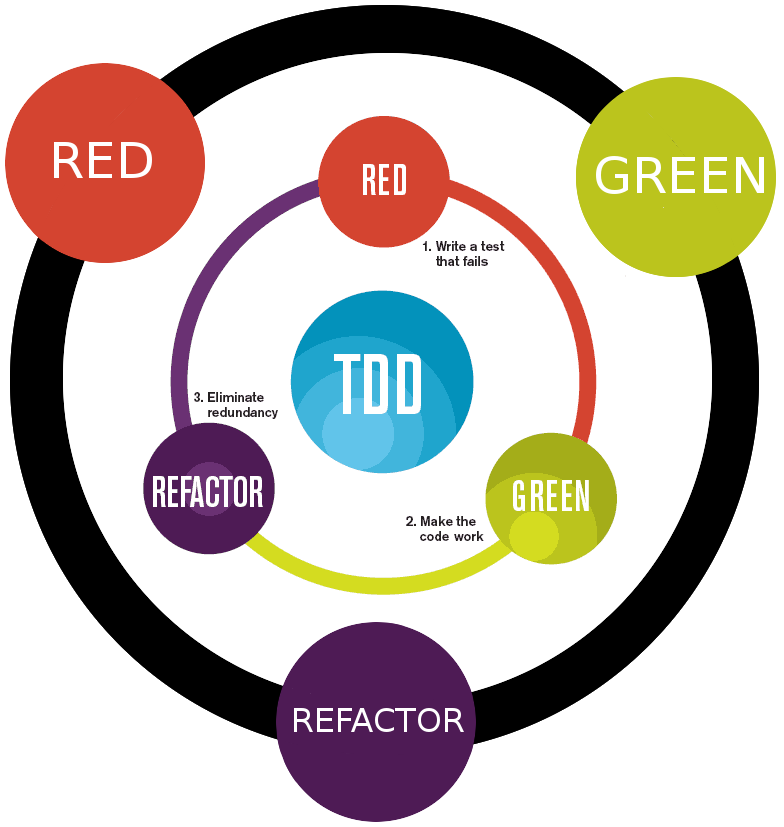
\includegraphics[scale=0.3]{assets/bdd_flow.png}
      \end{center}
      \caption{BDD-Workflow}
      \vspace{-15pt}
    \end{wrapfigure}
    Dieser "au"ser Zyklus bedeutet nichts anderes als das Stakeholder Stories
    definieren um Verhalten der Software zu spezifizieren und sie somit bestimmen
    wann alle Stories 'gr"un' sind. Die Entwickler\_innen haben nun die M"oglichkeit sich einfach Feature f"ur Feature an den Stories der Stakeholder entlang zu 
    hangel und diese nacheinander zu Implementieren. Dabei werden bis auf die 
    zeitliche L"ange eines Features die gleichen Ma"sgaben wie bei TDD beachtet.\\
    Der innere Zyklus kommt nur zustande, falls die Features definierten Features
    von den Stakeholdern komplexer gew"ahlt sind. Dann k"onnen die Entwickler 
    diese nach TDD Prinzipien entwickeln und somit am Schluss sicher seien 
    dass ihr entwickeltes Feature minimal ist und trotzdem das gew"unschte 
    Verhalten repr"asentiert.\\

  \subsection{Beispiel: Umsetzung mit Cucumber/Rspec in Ruby}
    Am Beispiel einer Taschenrechner-Klasse in Ruby wollen wir nun die 
    Unterschiede zwischen Behaviour Driven Development und Test Driven 
    Development nachvollziehen.
    \subsubsection{TDD:}
      In TDD w"urden wir als erstes diese folgenden Tests spezifizieren 
      und dann die gew"unschten Features implementieren.
      \lstinputlisting[caption=Ruby UnitTest,firstline=5]{../tests/calculator_test.rb}

    \subsubsection{BDD:}
      In BDD hingegen w"urden wir als erstes Stories f"ur das gew"unschte
      Verhalten schreiben und f"ur diese dann auch die passenden Step-Definitionen
      wie in Listing 1.1 und 1.2 gezeigt.\\
      Danach w"urden wir die gew"unschten Features implementieren und diese
      falls es die Komplexit"at verlangt nochmal einzeln in TDD entwickeln.\\
      Die genutzte Toolchain w"are Cucumber f"ur BDD und RSpec f"ur TDD.\\\\
      Ein Beispiel Projekt, sowie diese Arbeit sind zu finden auf 
      \href{http://github.com/bigzed/proseminar-bdd}{github/bigzed}.

  \subsection{Anderere Sprachen, andere Tools}
    Falls BDD in anderen Sprachen verfolgt werden soll gibt es hier eine nicht
    vollst"andige Liste mit anderen g"angigen Tools:
    \begin{itemize}
      \item Java -> \href{http://jbehave.org/}{JBehave}
      \item C -> \href{http://code.google.com/p/cbehave/}{CBehave}
      \item Ruby -> \href{http://cukes.info}{Cucumber}, \href{http://rspec.info}{RSpec}
      \item PHP -> \href{http://behat.org}{behat}
      \item Python -> \href{http://lettuce.it}{Lettuce}
    \end{itemize}
\section{Zusammenfassung}
  


\bibliographystyle{plain}
\bibliography{literature}
\end{document}
